% !TEX root =  ../main.tex
\chapter{Étude d'un premier ordre par les 4 méthodes de discrétisation.}

%===============================================================
\section{Introduction}
%===============================================================

Durant la première séance de laboratoire, il nous a été demandé de calculer l'expression récurrente d'un premier ordre par les 4 méthodes de discrétisation, à savoir : 
\begin{itemize}
\item La méthode de Euler 1 ;
\item La méthode de Euler 2 ;
\item La méthode bilinéaire ;
\item La méthode équivalent échantillonné bloqué.
\end{itemize}
Une fois les 4 expressions calculées, l'objectif était d'utiliser le logiciel MATLAB afin de représenter les réponses temporelles et fréquentielles de ces 4 expressions. Ceci, dans le but d'analyser les différents paramètres de ces 4 méthodes de discrétisation.


%===============================================================
\section{Rappels théoriques}
%===============================================================

\subsection{Discrétisation d'un signal}
%------------------------------------------------

Actuellement, les méthodes de traitements numériques pour l'analyse des signaux ont largement pris le dessus comparé aux méthodes analogiques ancestrales. C'est pourquoi nous abordons les notions de procédés de discrétisation. 
\paragraph{}
En effet, en traitement numérique, un signal analogique est tout d'abord échantillonné (= discrétisé) avant d'être quantifié et finalement codé. \textbf{La discrétisation est le procédé par lequel un signal continu est transformé en un signal discret}. Autrement dit, la discrétisation d'un signal continu f(t) revient à garder un certain nombre de valeurs discrètes (..., f($t_{0}$), f($t_{1}$), f($t_{2}$), ...) correspondant aux valeurs (..., $t_{0}$, $t_{1}$, $t_{2}$, ...) de la variable $t$. On parle également d'échantillonnage pour les signaux. Les différentes valeurs discrètes (..., f($t_{0}$), f($t_{1}$), f($t_{2}$), ...) varient en fonction de la période d'échantillonnage. La figure \ref{échantillonnage} ci-dessous présente le principe d'échantillonnage.
\begin{figure}[!ht]
\centering
	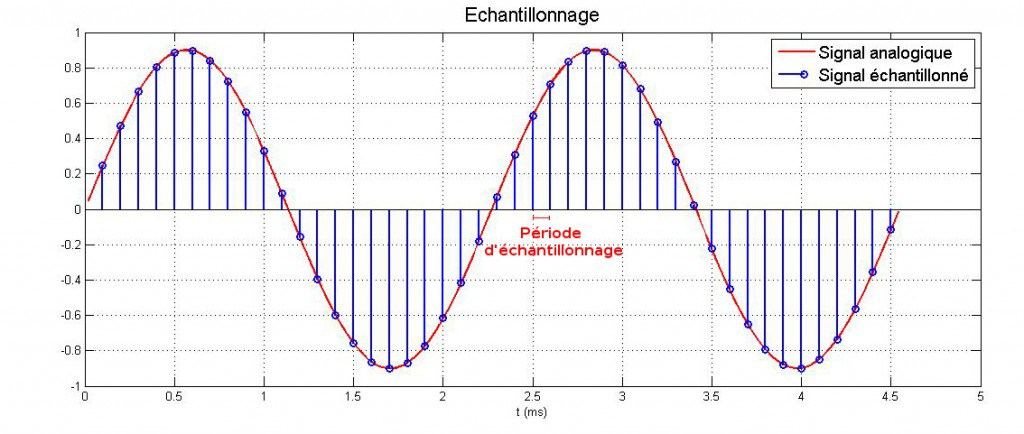
\includegraphics[scale=0.45]{images/echantillonnage.jpg}
	\caption{Échantillonnage d'un signal continu sinusoïdal.}
	\label{échantillonnage}
\end{figure}

\newpage
\subsection{Liens entre les domaines continu et discret}
%------------------------------------------------

En temps continu, nous pouvons travailler avec la transformée en $s$ d'un signal, qui nous amène dans le plan complexe.

En temps discret, nous travaillons avec la transformée en $z$ du signal et le plan $z$ qui comprend un cercle trigonométrique unitaire.

\paragraph{}
Le lien entre les grandeurs $s$ et $z$ est le suivant:
\begin{equation}
z = e^{hs} = e^{(\sigma + j\omega)h} = e^{\sigma h}e^{j\omega h}
\end{equation}
où h correspond à la période d'échantillonnage du signal.
\paragraph{}
On peut également réécrire $z$ sous la forme complexe suivante:
\begin{equation}
r = e^{\sigma h}, 
\Omega = \omega h \rightarrow
z = re^{j\Omega}
\end{equation}
où,
\begin{itemize}[label=$\cdot$]
\item $0\leq r\leq \infty$, le rayon, correspond au \textbf{facteur d'amortissement}
\item $-\pi \leq \Omega \leq \pi$, l'angle (radians), est la \textbf{pulsation discrète}
\end{itemize}

\paragraph{}
Dès lors, le lien entre le plan complexe de Laplace et le plan en z est celui donné à la figure \ref{labo1-lien-plans}.
\begin{figure}[!h]
\center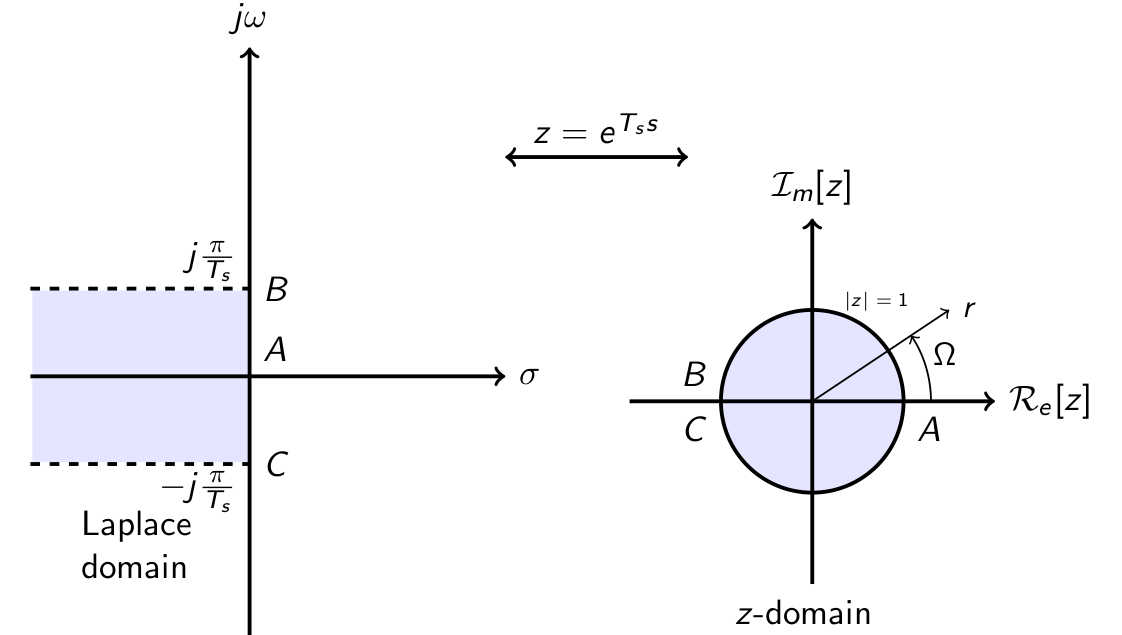
\includegraphics[scale=.2]{images/lien-plans}
\caption{Correspondance des plans $s$ et $z$}
  \small\textit{Signal and Systems: Z-transform}, F. De Bruyne
  \label{labo1-lien-plans}
\end{figure}
\paragraph{}
Nous pouvons en déduire que la stabilité d'un système, qui s'obtient par l'analyse de la position de ses pôles dans les domaines d'existence, est définie par:
\begin{itemize}[label=$\cdot$]
\item en continu: des pôles dans la partie gauche du plan
\item en discret: des pôles à l'intérieur du cercle unitaire
\end{itemize}

\newpage
%===============================================================
\section{Analyse d'un système de 1$^{er}$ ordre}
%===============================================================
Nous allons maintenant présenter la discrétisation (suivant les méthodes citées précédemment) du système de 1$^{er}$ ordre dont la fonction de transfert est la suivante: 
\begin{equation*}
H(s)=\frac{1}{s+1}
\end{equation*}

\paragraph{}
Ce système en continu est stable puisqu'il possède un pôle en $s=-1$, et sa réponse indicielle est donc un signal qui se stabilise autour d'une valeur finie après $5*\tau$ ($\tau=1$\textit{sec} étant la constante de temps du système) soit 5sec dans notre cas. \\
Comme le pôle est projeté en discret selon l'expression $z=e^{sh}$, sa position est directement liée à la période d'échantillonnage du système. Nous verrons que selon la méthode utilisée, la projection de $s$ dans $z$ varie, ce qui peut rendre le système instable (selon la méthode et le h).

\paragraph{Remarque: } le code Matlab utilisé se trouve à l'annexe \ref{annexe-1}.

\subsection{Méthode de Euler 1 - Différences finies à gauche}
%------------------------------------------------

La discrétisation s'obtient en remplaçant $s$ par $\frac{z-1}{h}$ dans l'expression du système.

\paragraph{Résolution par voie analytique:}
\begin{equation}
\begin{split}
H(s) & = \frac{1}{s+1} \\
	& = \frac{1}{\frac{z-1}{h}+1} \\
	& = \frac{h}{z-1+h}
\end{split}
\end{equation}

\begin{figure}[!ht] 
  \begin{minipage}[b]{0.7\linewidth}
  La projection du pôle dans le domaine discret est donc:
	\begin{equation*}
	P_{z} = 1 - h
	\end{equation*}
	\paragraph{}
  Dès lors, puisque $h>0$ il vient que le pôle $z_{p}$ se trouve forcément dans le plan $z$ à gauche de la verticle en 1 et qu'il est possible d'obtenir un système instable.
  \end{minipage}%%
  \begin{minipage}[b]{0.3\linewidth}
    \centering
    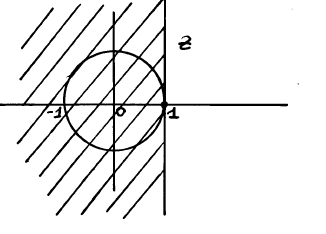
\includegraphics[scale=.6]{images/labo1-dom-gauche} 
   \end{minipage} 
\end{figure}

\newpage
\paragraph{Prévisions des valeurs particulières du pôle:}
\begin{itemize}[label=$\cdot$]
\item $h=0 \rightarrow z_{p}=1$: limite de stabilité du système discret
\item $h=1 \rightarrow z_{p}=0$: système discret stable à temps minimum
\item $h=2 \rightarrow z_{p}=-1$: limite de stabilité du système discret
\item $h>2 \rightarrow z<-1$: le système est instable
\end{itemize}
\paragraph{}
Via les résultas du script Matlab, nous voyons que nous obtenons bien les prévisions analytiques attendues. La méthode des différences finies à gauche engendre un système à temps minimum pour une période d'échantillonnage $h=1$ (pôle $z_{p} = 0$). Autrement dit, lorsqu'on applique un signal en entrée, la sortie atteint sa valeur finale directement après une période d'échantillonnage (fig. \ref{gaude-tempsmin}).

\begin{figure}[!h] 
  \label{ fig7} 
  \begin{minipage}[b]{0.5\linewidth}
    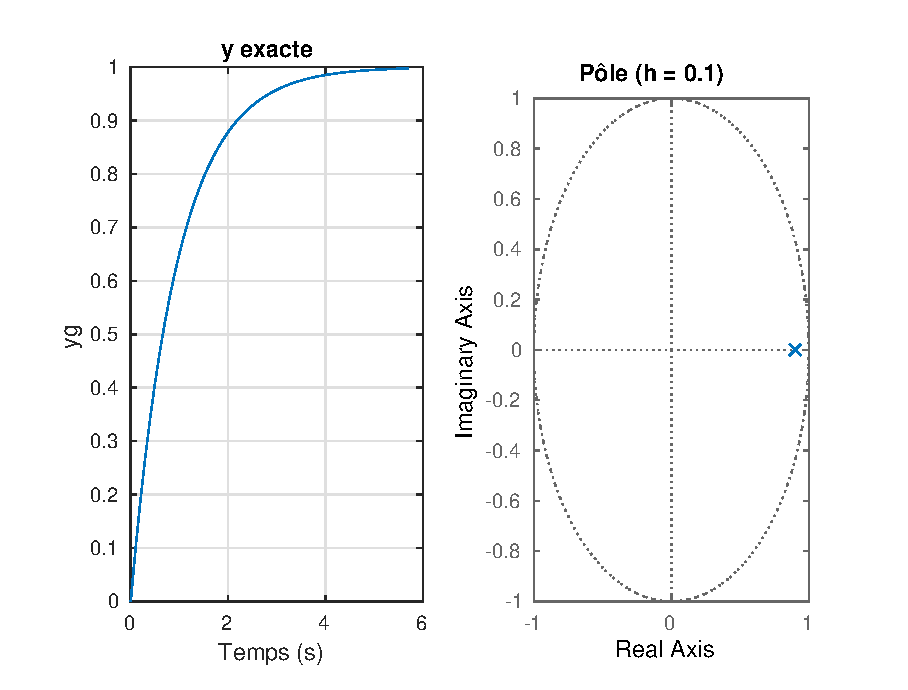
\includegraphics[width=1\linewidth]{eps/labo1-yg-0-1} 
    \caption{h = 0.1} 
    \vspace{4ex}
  \end{minipage}%%
  \begin{minipage}[b]{0.5\linewidth}
    \centering
    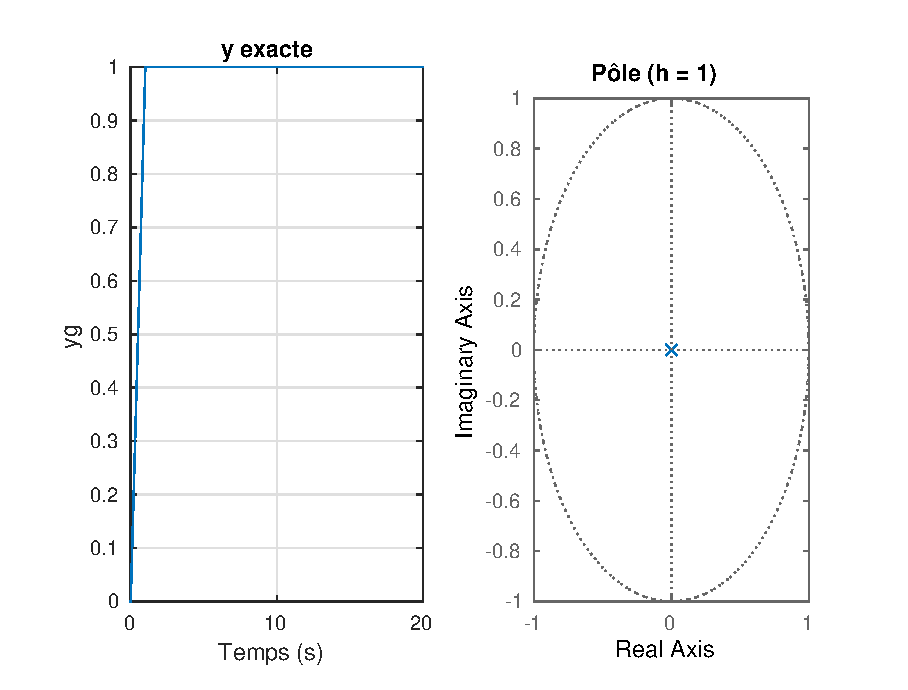
\includegraphics[width=1\linewidth]{eps/labo1-yg-1} 
    \caption{h = 1} 
        \label{gaude-tempsmin}
    \vspace{4ex}
  \end{minipage} 
  \begin{minipage}[b]{0.5\linewidth}
    \centering
    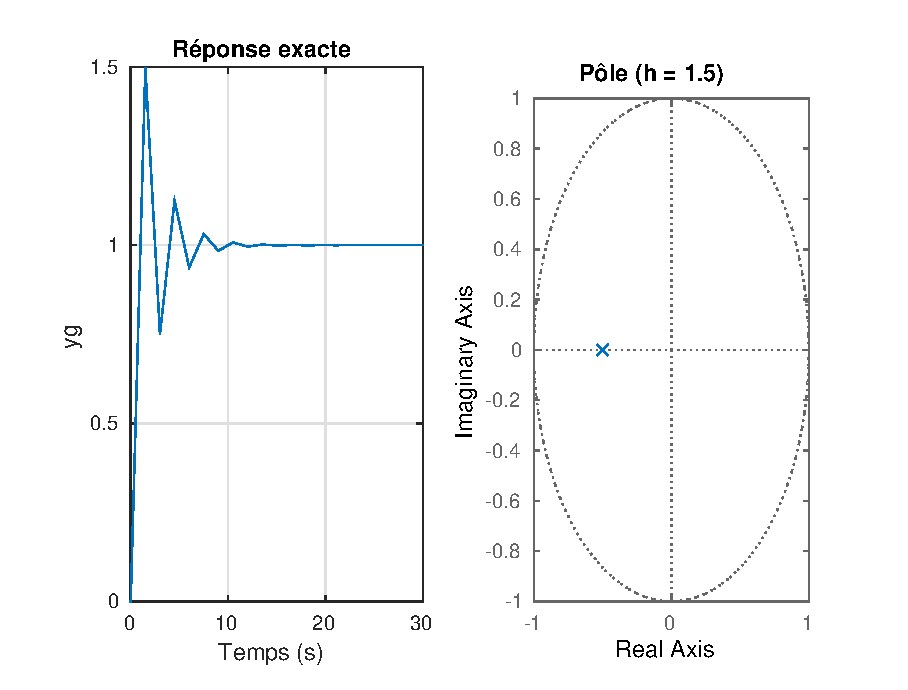
\includegraphics[width=1\linewidth]{eps/labo1-yg-1-5} 
    \caption{h = 1.5} 
    \vspace{4ex}
  \end{minipage}%% 
  \begin{minipage}[b]{0.5\linewidth}
    \centering
    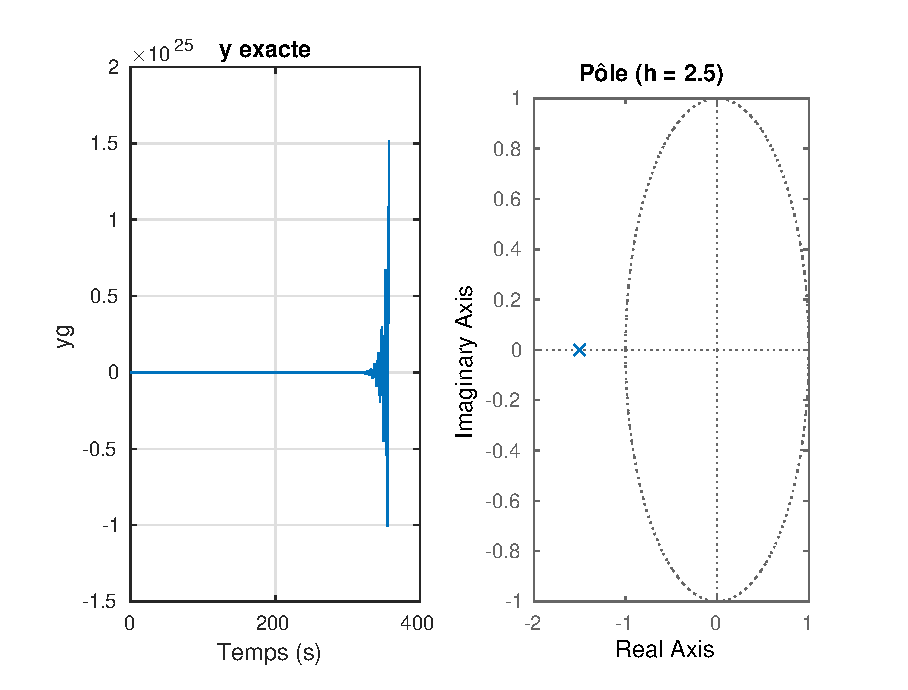
\includegraphics[width=1\linewidth]{eps/labo1-yg-2-5} 
    \caption{h = 2.5} 
        \label{gauche-instabilite}
    \vspace{4ex}
  \end{minipage} 
\end{figure}

\paragraph{}
En augmentant la période d'échantillonnage, on constate bien que le pôle se déplace vers la gauche et qu'il quitte le cercle lorsque cette période dépasse 2\textit{sec}. Le système fini alors par être en instabilité et le signal de sortie diverge (fig. \ref{gauche-instabilite}).

\paragraph{}
Nous pouvons voir sur la figure \ref{labo1-gauche-step} la comparaison du système discrétisé (h=0.1) avec sa réponse exacte. Pour cette période d'échantillonnage, nous obtenons un équivalent discret qui correspond bien au système réel, avec une erreur relative inférieure à 2\% \footnote{Les courbes des systèmes discrétisés sont approximées à partir des valeurs des échantillons}.

\begin{figure}[!h]
\center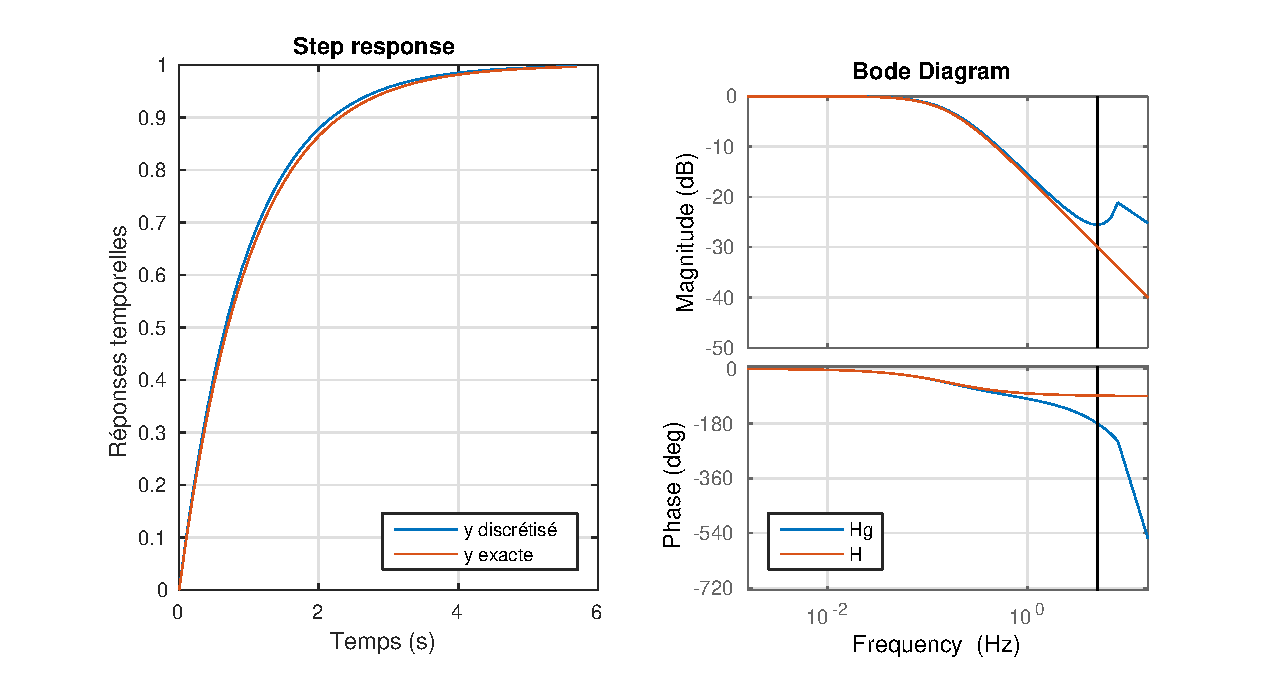
\includegraphics[width=1\linewidth]{eps/labo1-gauche-step}
\caption{Comparaison du système discrétisé et de sa réponse exacte en temporel et en fréquentiel, pour une période d'échantillonnage h=0.1 (Euler 1)}
\label{labo1-gauche-step}
\end{figure}

\paragraph{}
En fréquentiel, nous constatons que le signal discrétisé suit bien le système réel, au moins jusqu'à la fréquence de coupure de 1Hz. Une verticale est présente à 5Hz, dont nous reparlerons à la section \ref{labo1-comparaison}

\newpage
\subsection{Méthode de Euler 2 - Différences finies à droite}
%------------------------------------------------

La discrétisation s'obtient donc en remplaçant $s$ par $\frac{z-1}{zh}$ dans l'expression du système.

\begin{minipage}[b]{0.65\textwidth}
   La projection du pôle dans le domaine discret se trouve à l'intérieur d'un cercle, dans le cercle unitaire lui-même. Dès lors, il est impossible d'obtenir un système instable en le discrétisant par cette méthode.
\end{minipage}\hfill
\begin{minipage}[c]{0.3\textwidth}
  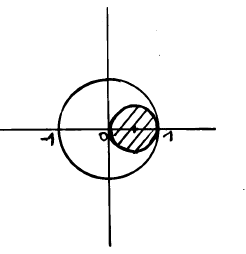
\includegraphics[scale=.6]{images/labo1-dom-droite} 
\end{minipage}

\begin{figure}[!h]
\center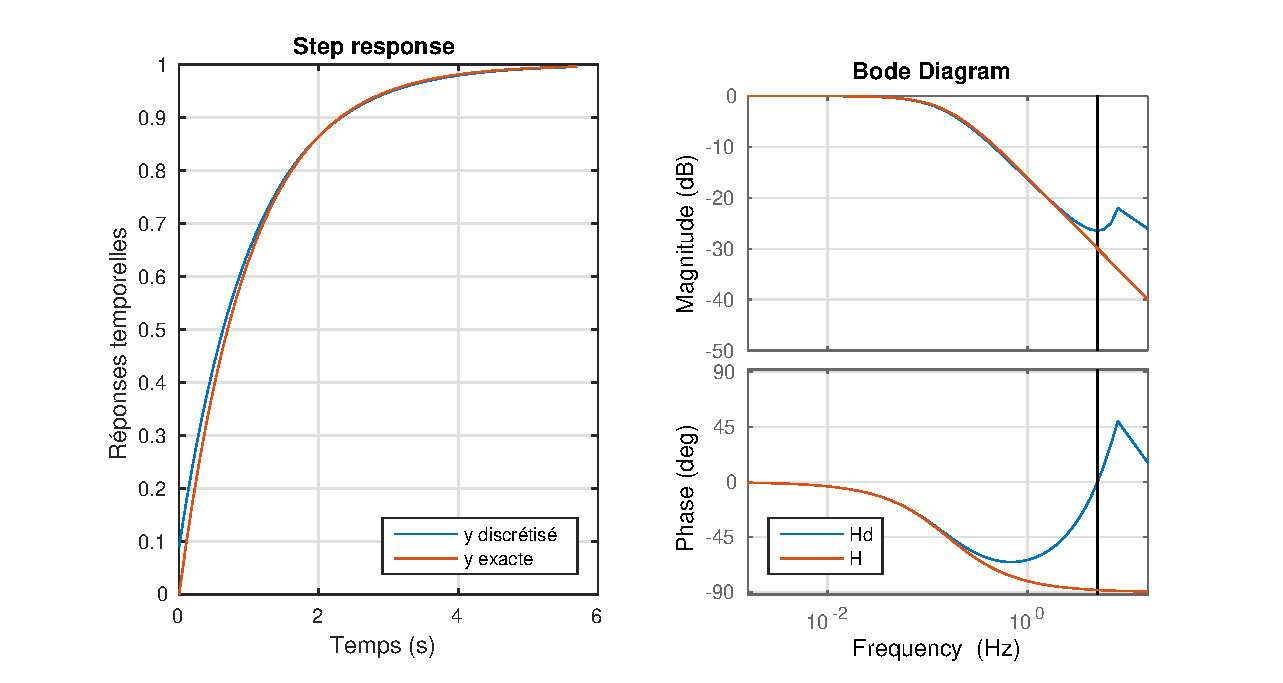
\includegraphics[width=1\linewidth]{eps/labo1-droite-step}
\caption{Comparaison du système discrétisé et de sa réponse exacte en temporel et en fréquentiel, pour une période d'échantillonnage h=0.1 (Euler 2)}
\label{labo1-droite-step}
\end{figure}


\subsection{Méthode bilinéaire - Différences finies centrales (Tustin)}
%------------------------------------------------
 
La forme discrète du système est obtenue en remplaçant $s$ par son approximation en $z$:  $s=\frac{2}{h}*\frac{z-1}{z+1}$, ou encore
\begin{equation}
z = \frac{1+\frac{j\omega h}{2}}{1-\frac{j\omega h}{2}}
\end{equation}

\begin{minipage}[b]{0.65\textwidth}
Pour une telle méthode, la projection des pôles se retrouvera toujours à l'intérieur du cercle unitaire lui-même. De nouveau, il est impossible que le système devienne instable suite à sa discrétisation.
\end{minipage}\hfill
\begin{minipage}[c]{0.3\textwidth}
  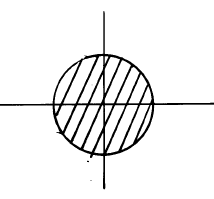
\includegraphics[scale=.6]{images/labo1-dom-centre} 
\end{minipage}

\begin{figure}[!h]
\center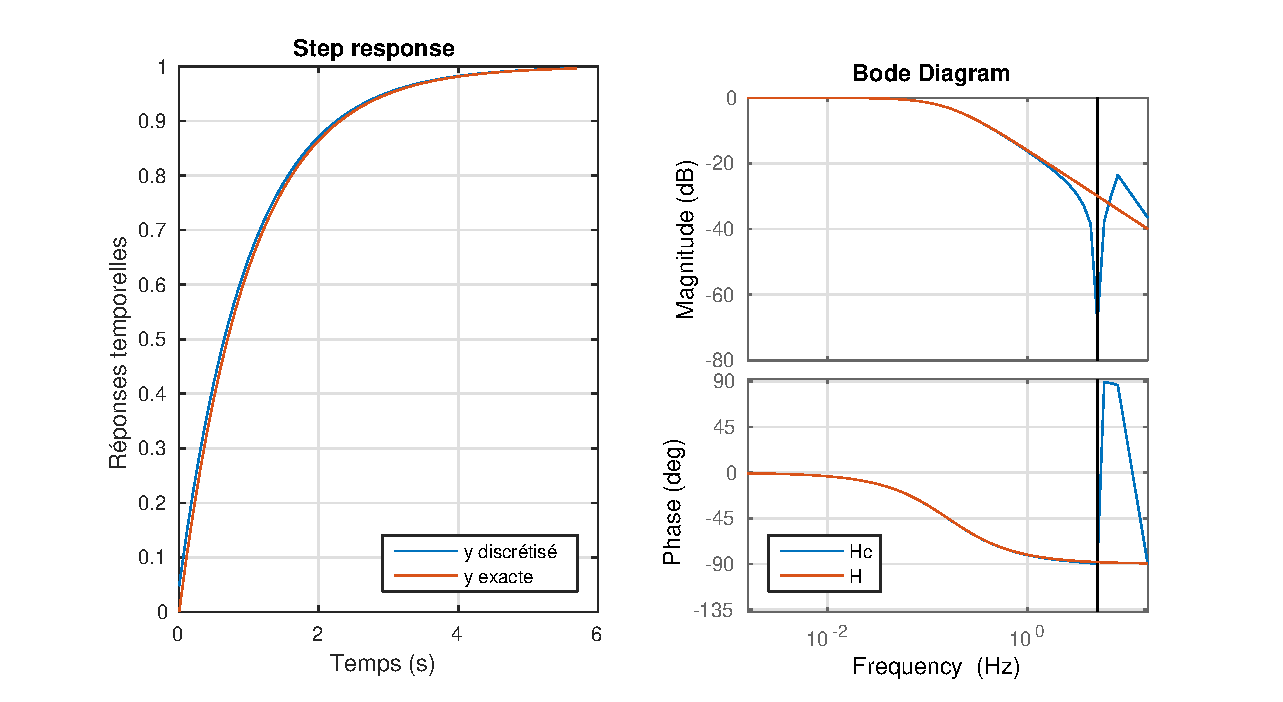
\includegraphics[width=1\linewidth]{eps/labo1-centre-step}
\caption{Comparaison du système discrétisé et de sa réponse exacte en temporel et en fréquentiel, pour une période d'échantillonnage h=0.1 (Bilinéaire)}
\label{labo1-centre-step}
\end{figure}


\subsection{Méthode de l'équivalent échantillonné bloqué}
%------------------------------------------------

Cette méthode utilise un bloqueur d'ordre 0 dont le but est de maintenir en sortie une valeur pendant l'équivalent d'une période d'échantillonnage, après quoi il change la sortie pour la nouvelle valeur qu'il a reçue. La sortie de ce bloqueur est "en moyenne" en retard sur l'entrée d'une demi-période.
\paragraph{}
De plus, sa sortie à une impulsion discrète en entrée est un "palier" de la même amplitude qui est maintenu pendant une durée $h$.

\paragraph{}
Comme nous le constatons à la figure \ref{labo1-bloque-step}, la sortie indicielle du système discrétisé par cette méthode est confondue avec celle du système réel.

\begin{figure}[!h]
\center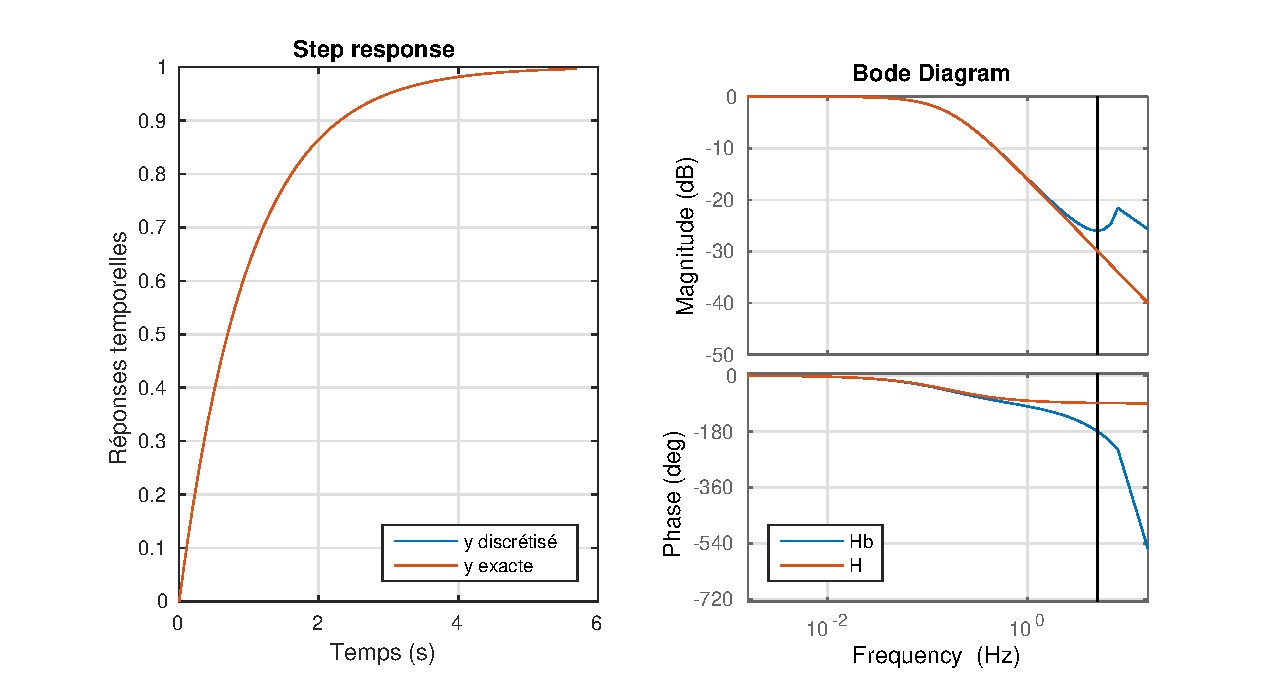
\includegraphics[width=1\linewidth]{eps/labo1-bloque-step}
\caption{Comparaison du système discrétisé et de sa réponse exacte en temporel et en fréquentiel, pour une période d'échantillonnage h=0.1 (Equiv bloqué)}
\label{labo1-bloque-step}
\end{figure}


%===============================================================
\section{Comparaison des méthodes de discrétisation}\label{labo1-comparaison}
%===============================================================
\subsection{Analyse fréquentielle}
L'analyse des systèmes discrétisés en fréquentiel nous permet de voir qu'ils ont bien tous une fréquence de coupure à $\frac{1}{2\pi}$Hz, qui est bien la fréquence de coupure d'un simple système de 1$^{er}$ ordre avec comme constante de temps $\tau=1$\textit{sec}

\paragraph{}
De plus, sur les figures \ref{labo1-comp-bode-10} et \ref{labo1-comp-bode-1}, nous observons la présence d'une verticale, au-delà de laquelle les signaux discrétisés changent d'aspect.
\paragraph{}
Dans le cas d'un signal discrétisé, il y aura toujours une telle verticale qui se retrouve à la demi-fréquence d'échantillonnage. Au delà de celle-ci le signal "ne veut plus rien dire" et cela s'explique par le théorème de Nyquist-Shanon qui nous dit "\textit{qu'il est impératif d'échantillonner un signal à une fréquence au moins supérieure (ou égale) au double de la fréquence maximale contenue dans le signal}".
\paragraph{}
En dessous de cette verticale, nous sommes donc en bande de base et au-delà, nous obtenons les répétitions du spectre du signal aux multiples de la fréquence d'échantillonnage.

\begin{figure}[!h]
\centering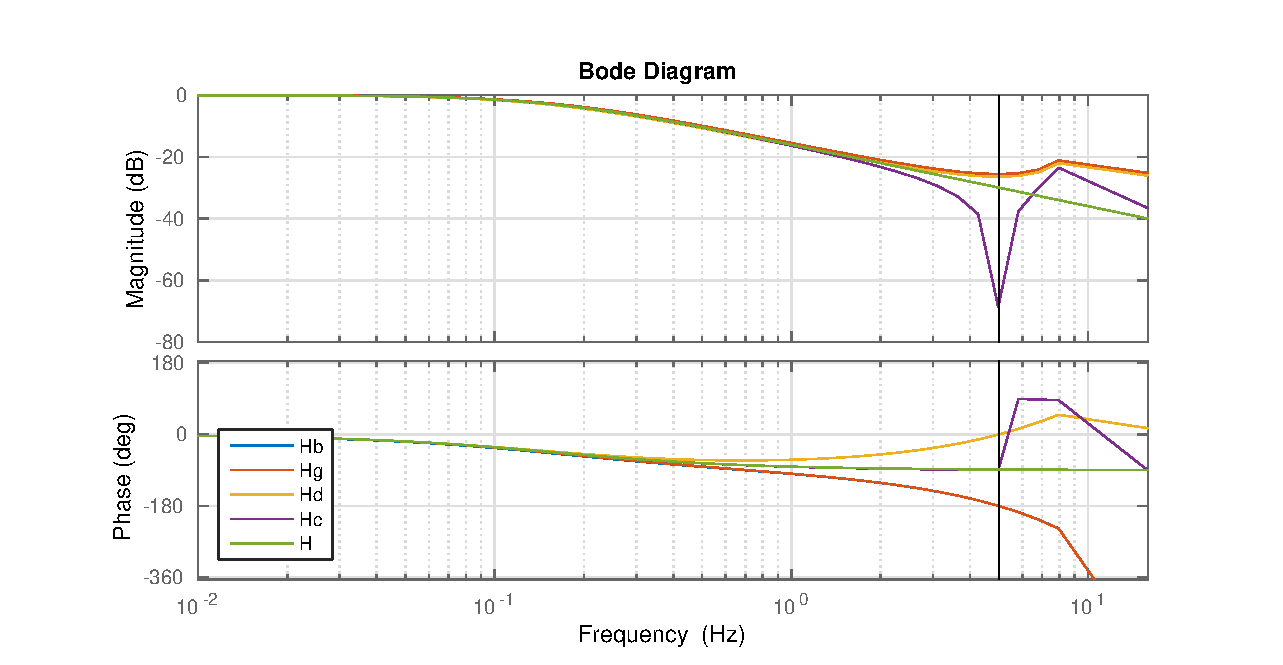
\includegraphics[scale=.9]{eps/labo1-comp-bode-0-1}
\caption{Discrétisation du système à une fréquence d'échantillonnage de 10Hz}
\label{labo1-comp-bode-10}
\end{figure}
\begin{figure}[!h]
\centering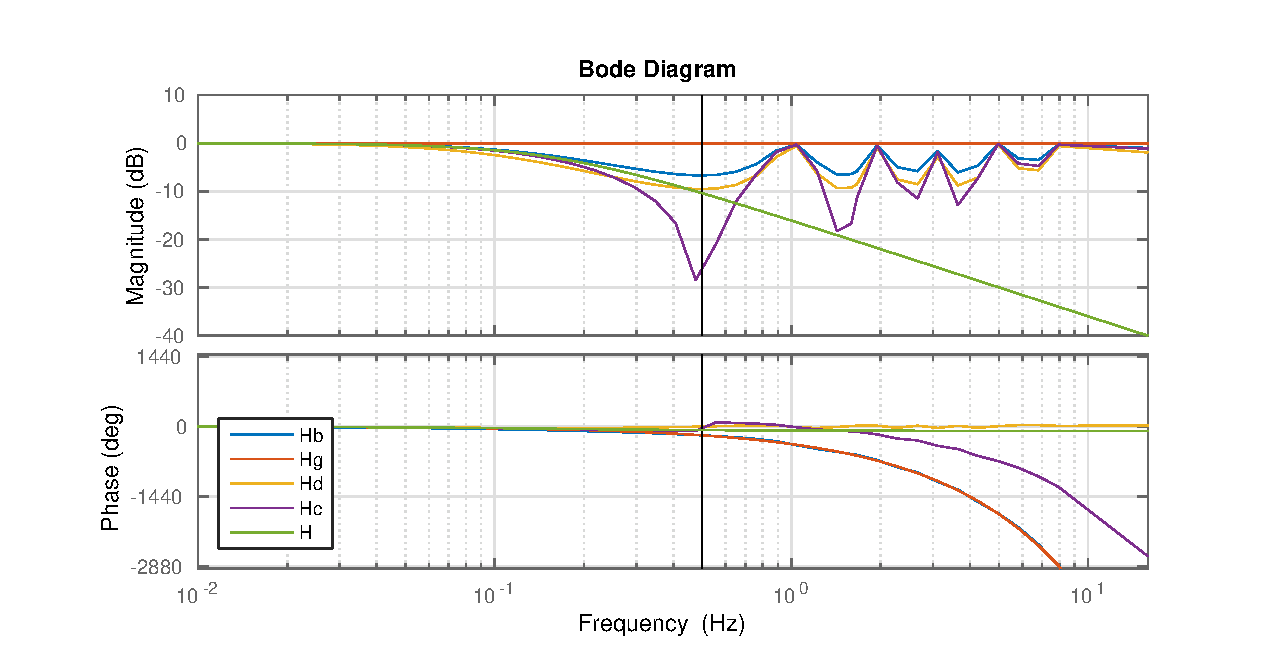
\includegraphics[scale=.9]{eps/labo1-comp-bode-1}
\caption{Discrétisation du système à une fréquence d'échantillonnage de 1Hz}
\label{labo1-comp-bode-1}
\end{figure}

\begin{table}[!h]\centering
\begin{tabular}{|c|c|c|}
\hline
 & Gain ($f_{ech}=10Hz$) & Gain ($f_{ech}=1Hz$) \\
\hline Système continu & Infini & Infini \\
\hline
Euler 1 (Diff gauche) & 19dB & 1dB\\
\hline
Euler 2 (Diff droite) & Infini & Infini \\
\hline
Bilinéaire (Diff centrale) & Infini & Infini \\
\hline
Equiv. bloqué & 20.02dB & 2.16dB\\
\hline
\end{tabular}
\end{table}

\subsection{Analyse temporelle}
L'analyse et la comparaison des réponses indicielles des systèmes discrétisés (h=0.1), nous permettent d'observer que ceux-ci s'éloignent très légèrement de l'allure du système réel. Après une constante de temps $\tau=1sec$, l'erreur passe en dessous de 2\% pour toutes les méthodes, et elle est pratiquement nulle une fois la stabilité atteinte.\paragraph{}
Lorsque la période d'échantillonnage augmente, le nombre d'échantillons diminuant, l'erreur augmente progressivement. Cela est d'autant plus vrai pour la méthode des différences finies à gauche.
\paragraph{}
Finalement, l'équivalent échantillonné bloqué présente une erreure relative qui est pratiquement nulle et ce quelle que soit la fréquence d'échantillonnage.

\begin{figure}[h]
	\begin{minipage}[b]{.5\linewidth}
	\centering
	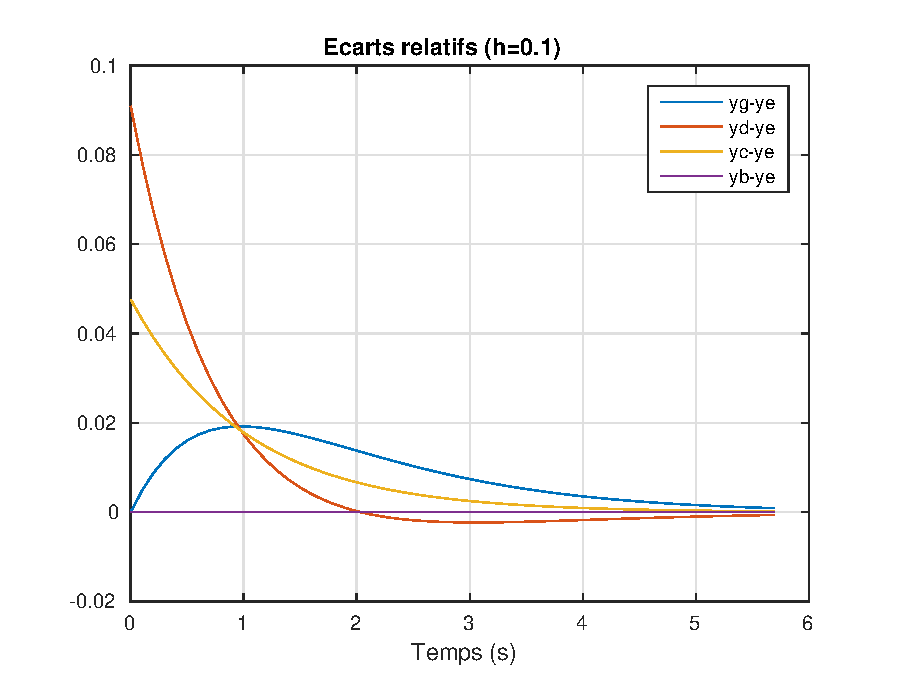
\includegraphics[scale=.6]{eps/labo1-ecarts-0-1}
	\end{minipage}
	\begin{minipage}[b]{.5\linewidth}
	\centering
	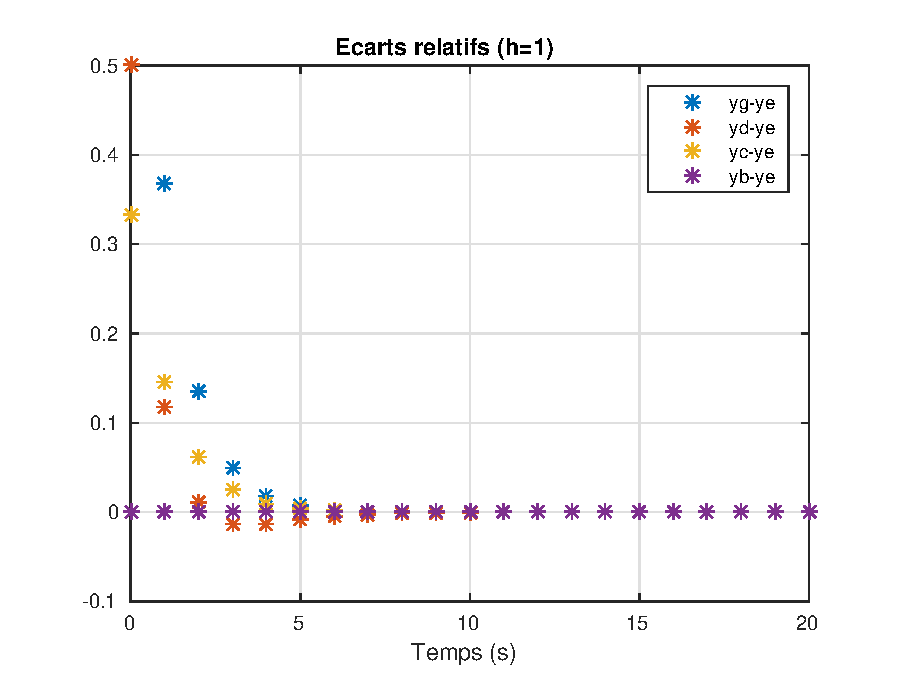
\includegraphics[scale=.6]{eps/labo1-ecarts-1}
	\end{minipage}
	\caption{Comparaison des écarts relatifs entre le système réel et les systèmes discrétisés.}
\label{labo1-ecarts}
\end{figure}


%===============================================================
\section{Conclusion}
%===============================================================
\begin{enumerate}
\item Le résultat obtenu par la méthode de l'\textbf{équivalent échantillonné bloqué} est la plus satisfaisante, c'est celle qui permet d'obtenir le système discret avec un comportement le plus proche du système réel.
\item Par la méthode des différences finies à gauche, des pôles dans la partie  gauche (système stable) du plan en continu peuvent être projetés en dehors du cercle dans le plan z et ce en fonction de la période d'échantillonnage. Dès lors, une telle discrétisation d'un système peut le rendre \textbf{instable}.
\item Lorsqu'on discrétise un système, il est important de prendre une période d'échantillonnage suffisament petite pour éviter le phénomène de repli spectrale.
\item Le gain critique d'un système du 1$^{er}$ ordre bouclé vaut l'infini car la courbe des phases est asymptotique à -90 et qu'on a toujours de la marge de phase.
\end{enumerate}

%===============================================================
\section{Analyse d'un système d'ordre 3}
%===============================================================
Soit le système suivant d'ordre 3 :
\begin{equation*}
H(s) = \frac{1}{(s+1)^{3}}
\end{equation*}

\paragraph{}
Nous allons étudier le déplacement de ce système discrétisé, en fonction de la période d'échantillonnage.

\paragraph{}
La fonction que nous obtenons pour le système discrétisé par la méthode d'échantillonneur bloqué (c2d) est la suivante:
\begin{itemize}[label=$\cdot$, itemsep=1em]
\item $h=0.1$
\begin{equation}
Hb(z) = \frac{0.0001547 z^{2} + 0.000574z + 0.0001331}{z^{3} - 0.406 z^{2} + 0.05495z - 0.002479}
\end{equation}

\item $h=1$
\begin{equation}
Hb(z) = \frac{0.0803 z^{2} + 0.1544z + 0.01788}{z^{3} - 1.104 z^{2} + 0.406z - 0.04979}
\end{equation}

\item ...
\end{itemize}

\paragraph{}
Nous voyons bien que la discrétisation du système d'ordre 3 fait apparaître au numérateur un second degré en $z$ et donc deux zéros dont la valeur varie avec la période d'échantillonnage.
\\Ces zéros restent dans la partie gauche du plan, peu importe la période d'échantillonnage, et ils sont ramenés à l'intérieur du cercle unitaire pour une période supérieure à 2\textit{sec}.
\begin{figure}[!h]  
  \begin{minipage}[b]{0.5\linewidth}
    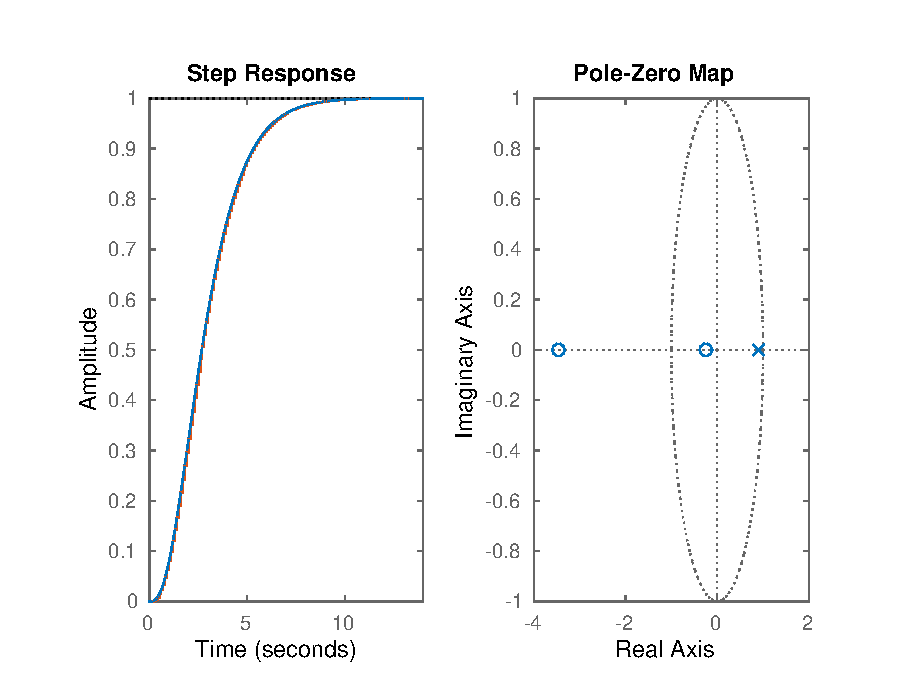
\includegraphics[width=1\linewidth]{eps/labo1-ordre3-0-1} 
    \caption{h = 0.1} 
    \vspace{4ex}
  \end{minipage}%%
  \begin{minipage}[b]{0.5\linewidth}
    \centering
    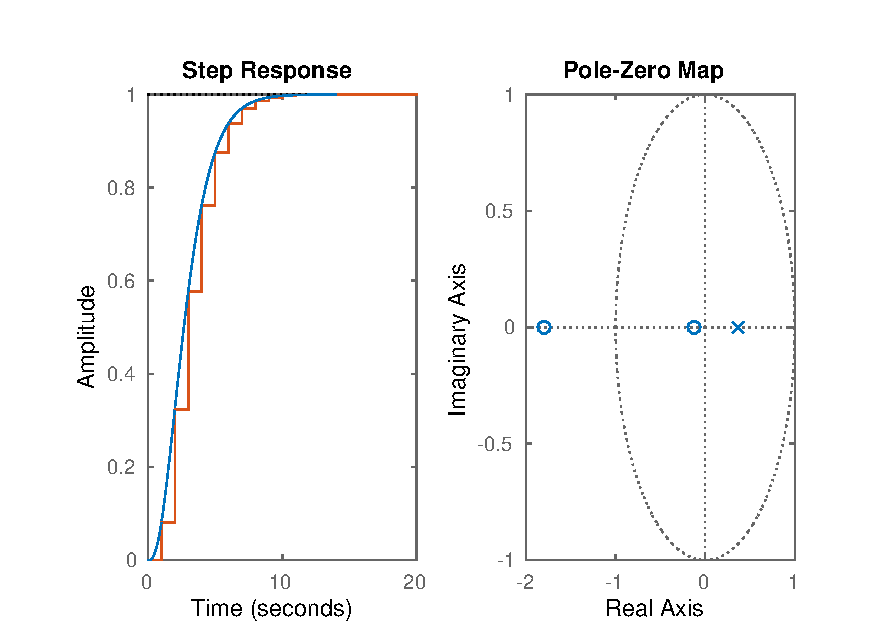
\includegraphics[width=1\linewidth]{eps/labo1-ordre3-1} 
    \caption{h = 1} 
    \vspace{4ex}
  \end{minipage} 
  \begin{minipage}[b]{0.5\linewidth}
    \centering
    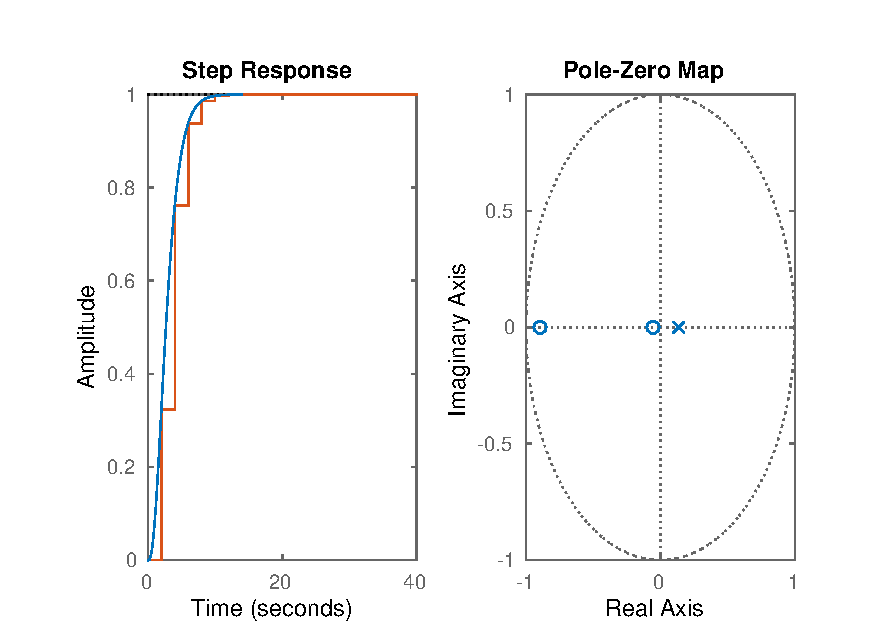
\includegraphics[width=1\linewidth]{eps/labo1-ordre3-2} 
    \caption{h = 2} 
    \vspace{4ex}
  \end{minipage}%% 
  \begin{minipage}[b]{0.5\linewidth}
    \centering
    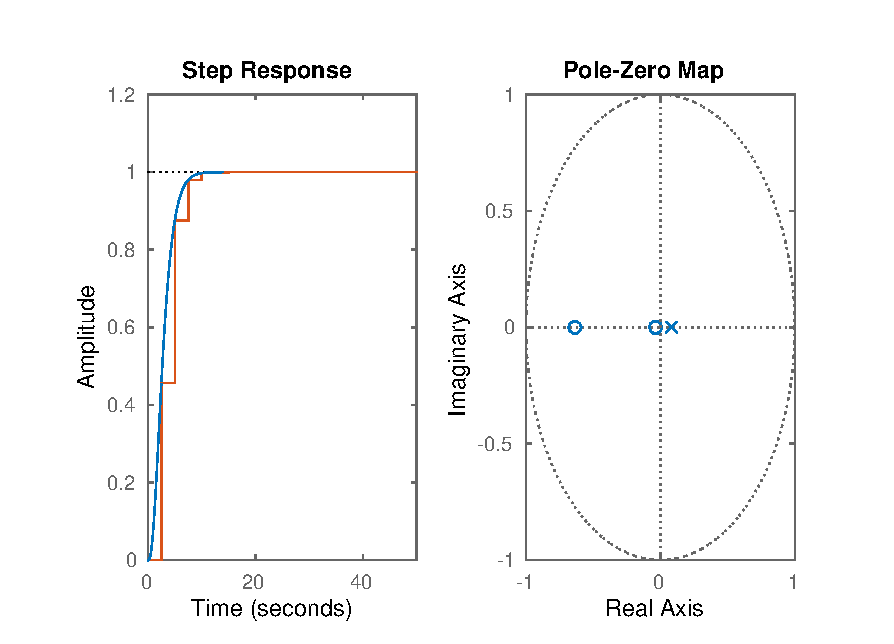
\includegraphics[width=1\linewidth]{eps/labo1-ordre3-2-5} 
    \caption{h = 2.5} 
    \vspace{4ex}
  \end{minipage} 
\end{figure}